\documentclass[tikz,border=8pt]{standalone}
\usetikzlibrary{arrows.meta,backgrounds,fit,positioning}

\definecolor{flowblue}{HTML}{D9EAF7}
\definecolor{flowgreen}{HTML}{D9EAD3}
\definecolor{flowred}{HTML}{F4CCCC}
\definecolor{flowyellow}{HTML}{FFF2CC}
\definecolor{flowline}{HTML}{4F6D7A}

\tikzset{
  step/.style={
    draw=flowline,
    rounded corners=2pt,
    fill=#1,
    minimum width=2.75cm,
    minimum height=1.0cm,
    align=center,
    font=\sffamily\small
  },
  step/.default=flowblue,
  data/.style={
    draw=flowline,
    rounded corners=2pt,
    fill=flowyellow,
    minimum width=2.35cm,
    minimum height=0.9cm,
    align=center,
    font=\sffamily\small
  },
  arrow/.style={-Latex,thick,draw=flowline},
  faint/.style={draw=flowline,rounded corners=4pt,dashed,inner sep=8pt}
}

\begin{document}
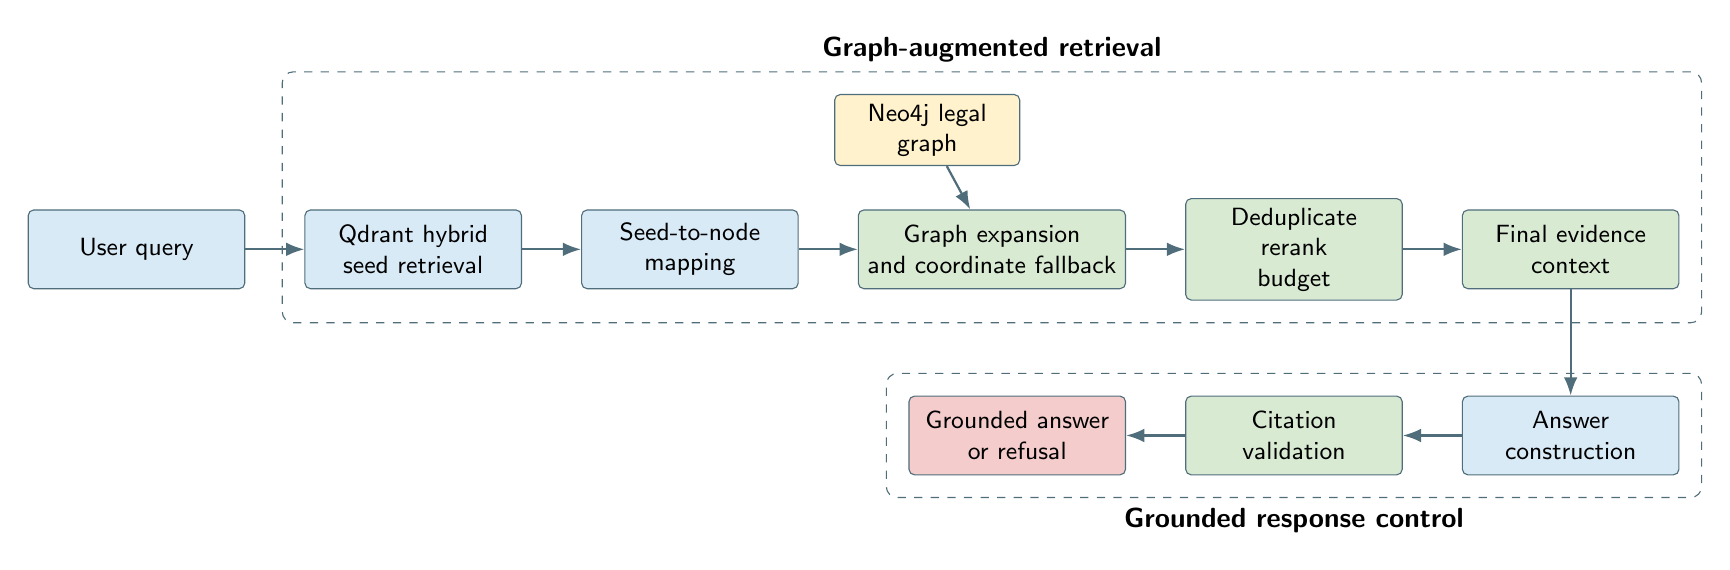
\begin{tikzpicture}[node distance=0.72cm and 0.75cm]
  \node[step=flowblue] (query) {User query};
  \node[step=flowblue, right=of query] (hybrid) {Qdrant hybrid\\seed retrieval};
  \node[step=flowblue, right=of hybrid] (map) {Seed-to-node\\mapping};
  \node[data, above right=0.55cm and 0.45cm of map] (graph) {Neo4j legal\\graph};
  \node[step=flowgreen, right=of map] (expand) {Graph expansion\\and coordinate fallback};
  \node[step=flowgreen, right=of expand] (rerank) {Deduplicate\\rerank\\budget};
  \node[step=flowgreen, right=of rerank] (context) {Final evidence\\context};
  \node[step=flowblue, below=1.35cm of context] (answer) {Answer\\construction};
  \node[step=flowgreen, left=of answer] (validate) {Citation\\validation};
  \node[step=flowred, left=of validate] (result) {Grounded answer\\or refusal};

  \draw[arrow] (query) -- (hybrid);
  \draw[arrow] (hybrid) -- (map);
  \draw[arrow] (map) -- (expand);
  \draw[arrow] (graph) -- (expand);
  \draw[arrow] (expand) -- (rerank);
  \draw[arrow] (rerank) -- (context);
  \draw[arrow] (context) -- (answer);
  \draw[arrow] (answer) -- (validate);
  \draw[arrow] (validate) -- (result);

  \begin{scope}[on background layer]
    \node[faint,fit=(hybrid)(map)(graph)(expand)(rerank)(context),label={[font=\sffamily\bfseries]above:Graph-augmented retrieval}] {};
    \node[faint,fit=(answer)(validate)(result),label={[font=\sffamily\bfseries]below:Grounded response control}] {};
  \end{scope}
\end{tikzpicture}
\end{document}
